\documentclass[10pt]{standalone}
\usepackage{amsmath}
\usepackage{amssymb}
\usepackage{grafica}
\usepackage{mathrsfs}
\usetikzlibrary{arrows,calc,positioning,shapes.symbols,shapes.geometric,shapes.misc}
\pagestyle{empty}
\usepackage{siunitx}
\begin{document}

% Define a few constants for easy configuration
%\def\radius{2}
%\def\onedegrad{1.8}
%\def\fivedegrad{1.75}
%\def\tendegrad{1.7}
%\def\labelrad{1.6}

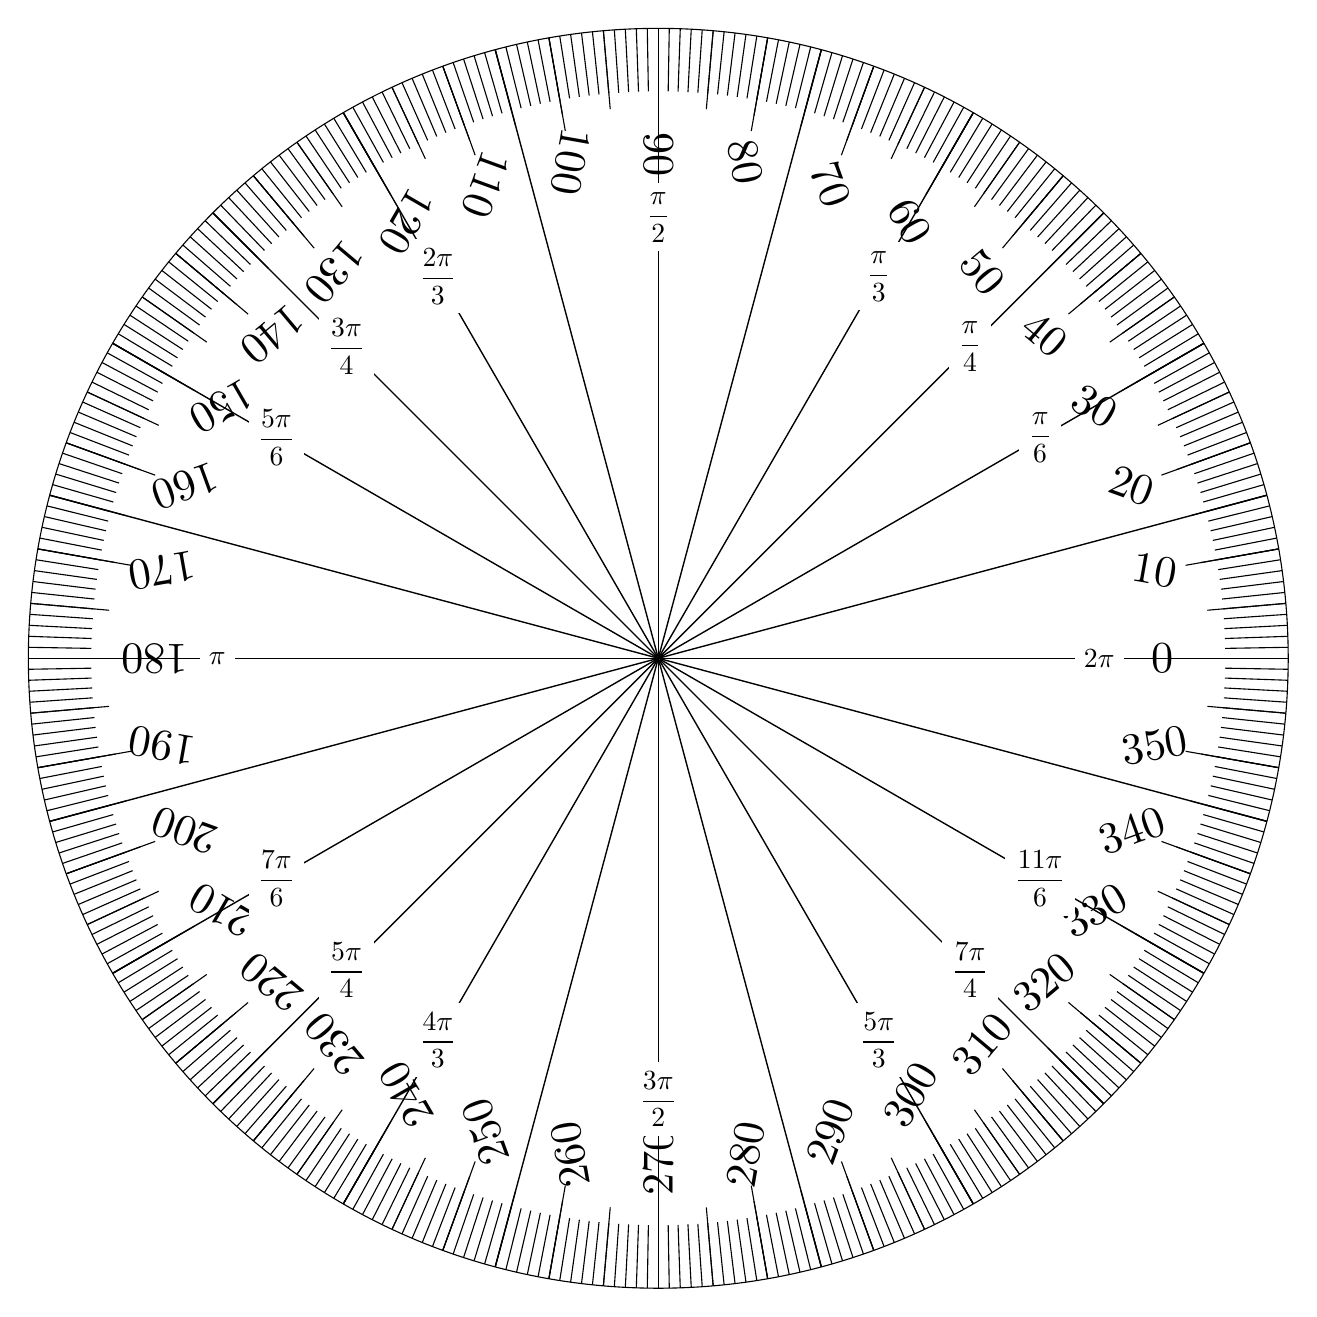
\begin{tikzpicture}%[scale=3.5]
\pgfmathsetmacro{\radius}{8};
\pgfmathsetmacro{\onedegrad}{\radius*0.9};
\pgfmathsetmacro{\fivedegrad}{\radius*0.875};
\pgfmathsetmacro{\tendegrad}{\radius*0.85};
\pgfmathsetmacro{\labelrad}{\radius*0.8};
\pgfmathsetmacro{\fscale}{\radius*0.2};
\pgfmathsetmacro{\fscal}{\radius*0.7};
% adding a subtle gray tone to add a bit of "personality"
\shade[shading=radial, inner color=white] (0,0) circle (\radius);

\draw (0,0) circle (\radius);
\draw[fill=black] (0,0) circle (.02);
\node[draw, circle, inner sep=.2] (a) at (0,0) {};

% helper lines
\foreach \x in {0, 15, ..., 360} \draw[very thin,line width=0.5pt] (a) -- (\x:\radius);
\foreach \x in {0,90 ,..., 360} \draw[very thin,line width=0.5pt] (a) -- (\x:\radius);
% main lines
\foreach \x in {0,...,359} \draw (\x:\onedegrad) -- (\x:\radius);

% labels and longer lines at every 10 degrees
\foreach \x in {0,10,...,350}
{
	\node[scale=\fscale, rotate=\x*-1] at (360+\x:\labelrad) {\x};
	\draw (\x:\tendegrad) -- (\x:\radius);
};
%\node(a1) at (-3,2) {  +};
%\node(a2) at (3,2) {SEN +};
%\node(a3) at (3,-2) {SEN -};
%\node(a4) at (-3,-3) {SEN -};
%\node(a5) at (3,3) {COS +};
%\node(a6) at (-3,3) {COS -};
%\node(a7) at (3,-1) {COS +};
%\node(a8) at (-3,-2) {COS -};
%\node(a9) at (3,1) {TAN +};
%\node(a10) at (3,-3) {TAN -};
%\node(a11) at (-3,1) {TAN -};
%\node(a12) at (-3,-1) {TAN +};
% lines at every 5 degrees
\foreach \x in {0,5,...,355}  \draw (\x:\fivedegrad) -- (\x:\radius);
\foreach \x/\xtext in {
	30/\dfrac{\pi}{6},
	45/\dfrac{\pi}{4},
	60/\dfrac{\pi}{3},
	90/\dfrac{\pi}{2},
	120/\dfrac{2\pi}{3},
	135/\dfrac{3\pi}{4},
	150/\dfrac{5\pi}{6},
	180/\pi,
	210/\dfrac{7\pi}{6},
	225/\dfrac{5\pi}{4},
	240/\dfrac{4\pi}{3},
	270/\dfrac{3\pi}{2},
	300/\dfrac{5\pi}{3},
	315/\dfrac{7\pi}{4},
	330/\dfrac{11\pi}{6},
	360/2\pi}
\draw (\x:\fscal) node[fill=white] {$\xtext$};
\end{tikzpicture}

\end{document}